\setlength{\columnsep}{3pt}
\begin{flushleft}
	\bigskip
	\begin{itemize}
		\item In older OS, network interfaces were named as eth0, eth1, eth2, and so on.
		\item New names of ethernet cards are assigned based on firmware, device topology, and device type. 
		\item Interface names have the following characters:
		\begin{itemize}
			\item The beginning character can be: 
			\begin{itemize}
				\item \textbf{en}: For ethernet interfaces.
				\item \textbf{wl}: For WLAN interfaces.
				\item \textbf{ww}: For WWAN interfaces.
			\end{itemize}
			\item The next character can be: 
			\begin{itemize}
				\item \textbf{o}: For on-board.
				\item \textbf{s}: For hotplug slot.
				\item \textbf{p}: For PCI geographic location
			\end{itemize}		
			\item Finally, a number N is used to represent an index, ID, or port.
		\end{itemize}
		\item Eg: A PCI card network interface may be named enp2s0.
		\begin{figure}[h!]
			\centering
			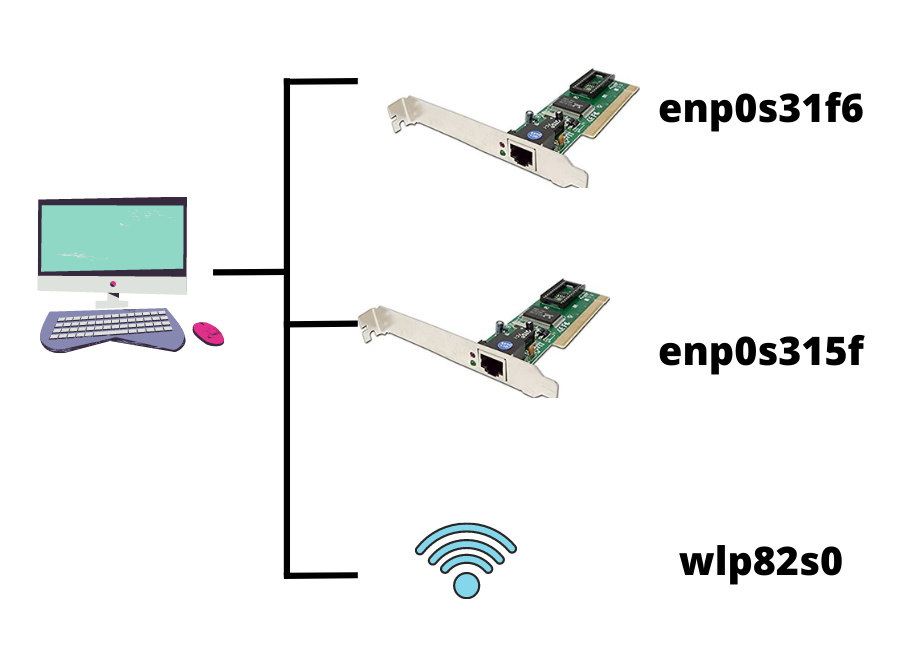
\includegraphics[scale=0.45]{content/chapter14/images/naming.png}
			\caption{Ethernet card names}
			\label{fig:severity266}
		\end{figure}			
		

	\end{itemize}
	
 \end{flushleft}
\newpage


